\documentclass{IEEEtran}
\usepackage[utf8]{inputenc}
\usepackage{authblk}
\usepackage{graphicx}
%\usepackage{natbib}
%\usepackage[backend=bibtex,style=verbose-trad2]{biblatex}
\title{Adaptive Execution of Particle Advection Workloads}
\author[*]{Kristi Belcher}
\author[*]{Hank Childs}
\author[**]{Dan the Ghost}
\affil[*]{University of Oregon}
\affil[**]{Oak Ridge National Lab}

\begin{document}
\maketitle
%
%%%%%%%%%%%%%ABSTRACT%%%%%%%%%%%%%%%%%%%%%%%%%%%%%%%%%%%
%%%%%%%%%%%%%%%%%%%%%%%%%%%%%%%%%%%%%%%%%%%%%%%%%%%%%%%%
\textbf{\textit{Abstract-} Particle Advection is a fundamental flow visualiation calculation with widely varying workloads. 
%
Determining the optimal architecture to run these workloads on is a critical consideration. 
%
In this study, we investigate the important tradeoffs that must be factored in when deciding how to best schedule the Particle Advection workloads on appropriate resources. 
%
Given this insight, our main contribution is a new algorithm which adapts execution: using the GPU to run relevant parts of the problem and then switching the targeted device according to how the workload evolves.
%
This algorithm is motivated by the observation that CPUs are sometimes able to better perform part of the overall computation since (1) this practice avoids latency times to the GPU and (2) CPUs operate at a faster rate when the workload can't take advantage of the threads on a GPU.
%
We evaluate our algorithm by running workloads that vary over data set, number of particles, number of steps taken, and number of GPU nodes.
%
We then compare our algorithm to traditional GPU-only and CPU-only approaches.
%
Our findings show X, Y, and Z.
%
The results of this study will help inform the Scientific Visualiaiton community about those architectures that give optimal performance at certain stages of the simulation run.}
%
%%%%%%%%%%%%%INTRODUCTION%%%%%%%%%%%%%%%%%%%%%%%%%%%%%%%%
%%%%%%%%%%%%%%%%%%%%%%%%%%%%%%%%%%%%%%%%%%%%%%%%%%%%%%%%%
\section{Introduction}
%
(1) Intro for particle advection. What it does, why it's useful. Streamline vs. FTLE?
%
Particle Advection is a fundamental scientific visualization algorithm that calculates the displacement of particles along a velocity field - cite. 
%
This algorithm is a key element of flow analysis, commonly used to compute streamlines, pathlines, stream surfaces, and even Finite-Time Lyapunov Exponents (FTLE) - cite.
%
Although Particle Advection is such an important calculation for vector field visualizaiton, implementing an efficient large-scale parallel Particle Advection computation remains a challenge.
%
Because particle trajectories can vary greatly, Particle Advection is a data dependent problem that requires variable computational resources to sucessfully trace the particle streams.
%
As simulations currently being studied require more and more data to produce meaningful results, visualization and analysis is being performed in situ - cite.
%
(i.e. visualization performed as the simulation is running, even using the same resources).
%
As simulations become larger, running programs like Particle Advection on modern supercomputers becomes a requirement for reasonable results.

(2) Intro for vtk-m. Talk about portable performance and hardware agnostic. Should mention varying architectures on supercomputers.
%
Modern supercomputers have varied computational capabilities that make tailoring algorithms to those architectures a priority.
%
The supercomputers that researchers must work with have widely differing architectures.
%
From modest computational power to very high computational power, with several architectures that lie in between - cite?.
%
Because of this trend, it is important to take into consideration the kind of architecture that a simulation code will be run on. 
%
Sometimes, however, it is not as simple as just one of these kinds of archtiectures for a specific code.
%
In order to more effectively harness the computation power available on a supercomputer, many research scientists are utilizing several different kinds of architectures at one time, during the same run of a simulation code.
%
This kind of hybrid computing requires that researchers tailor their codes to two (or more in some cases)  architectures at a time.
%
To help ease the transition of efficiently using multiple hardwares, VTK-m was created to provide a hardware agnostic framework that acts as a bridge between several different plateforms \cite{Camp13}.
%
VTK-m is an extension of VTK, with the addition of several many-core implementations for common visualization algorithms.
%
Figure 1 shows a pictoral representation of how VTK-m can be used - cite. 
%
Note that in (a) a developer must implement several versions of the application code: one for each desired harware platform.
%
In (b), the developer only has to implement one VTK-m program to be able to utilize any compatible architecture.
%
Portable performance sentence here.
%
supercomputers.

(3) What we hope to gain from this study. What the focus of the study is. More general description of goal of paper. 
Mention research question.
%
In this study, we analyze the performance impact of utilizing more than just one architecture during the same run of a VTK-m Particle Advection program.
%
We contribute a new Particle Advection algorithm which uses an oracle to determine, at runtime, whether the CPU or the GPU can best handle the current workload, switching to that particular device.
%
As the workload evolves, our algorithm can switch back and forth from CPU to GPU depending on which device's hardware resources can be best utilized.
%
We compare the performance between programs which uses either only the CPU or only the GPU to produce results and our program which adaptively selects a device during execution depending on the current state of the workload. 
%
Our algorithm is motivated by the observation that sometimes the workload can't take full advantage of GPU threads, leading to some sitting idle and wasting resources.
%
This would lead to the speculation that leaving the data on the CPU to be computed would perform better.
%
At other times, the workload may be much more able to fully load the GPU and take advantage of its hardware abilities.
%
In effect, our work explores the fundamental research question: \textbf{If faced with a Particle Advection problem, can adaptive execution give better performance than running the entire workload on either the CPU or the GPU?}

(4) Other important contribution of the paper. Why should we care? What this study means to overall community.
%
Other important contributions of this paper include the insights it provides for visualization scientists who are studying Particle Advection and other flow visualizaiton problems.
%
For example, in implementing an oracle to efficiently determine the best device to run the algorithm, we had to factor in several different characteristics of the current workload.
%
These characteristics included (1) number of particles left in the domain to advect, (2) how many times a particular particle has been switched to a different device, and (3) how many times a particular particle when back and forth from active queue to inactive queue.
%
These considerations were important for scultping an oracle that could best determine the appropriate device for the workload, and thus will give other researchers interesting insight into the factors that affect which architectures will be best.
%
The following sections describe our algorithm and results in more detail. 
%
(Could say more about what sections are)
%
%%%%%%%%%%%%RELATED WORK%%%%%%%%%%%%%%%%%%%%%%%%%%%%%%%%
%%%%%%%%%%%%%%%%%%%%%%%%%%%%%%%%%%%%%%%%%%%%%%%%%%%%%%%%
\section{Related Work}
There are a few papers that survey flow visualization that would be good to include (3 in the other paper).
%
From here you can talk about porting these flow visualization algorithms to GPUs and studies that focus on that (4,5,6,7,8,9,10,11)
%
Then mention Particle Advection specifically and how that pairs with parallel algorithms that are implemented on the GPU, CPU, and/or a cluster of the two.
%
That is mentioned in section 2, parts C and D in that one paper.
%
Look at those references and see if you can't use them here too.
%
Mention David Camp (Pugmire, Childs) papers. (Paper used above + others)
%
Other presentations on particle advection.
%
Could talk about the effects of hardware architecture on PA performance. (Section 2, parts C and D)
%
Should include something on CPU vs GPU performance and when one device is better than the other. (part D, others)
%
Perhaps go into more details on problems that are better for GPU hardware vs problems that are better for CPU hardware.
%
Mallony papers could help on this part...
%
%%%%%%%%%%%PROBLEM and ALGORITHM OVERVIEW%%%%%%%%%%%%%%%
%%%%%%%%%%%%%%%%%%%%%%%%%%%%%%%%%%%%%%%%%%%%%%%%%%%%%%%%
\section{Problem and Algorithm Overview}
Should include a Particle Advection Overview + OUR algorithm overview here. Maybe new section?
%
\subsection{Particle Advection Overview}
Particle Advection starts by displacing a particle for a short distance in a velocity field.
%
That particle will be advected from one location to another nearby.
%
This displacement is also known as an advection step.
%
After a series of advection steps, the integral curve can be observed by the total path, or sequence of advection steps from the initial location to the terminal location, that particle has traveled.
%
Because the advection steps must be calculated sequentially, advecting particles is a data dependent problem.
%
In other words, in order to calculate a particle's Nth location, we must know it's (N-1)th location.
%
Additionally, the number of advection steps for any given particle varies, adding more complexity to the problem.
%
For example, the particle could advect into a sink, go outside the problem domain, or meet some other kind of termination criteria.
%
In this study, our Particle Advection algorithm uses a parallelization-over-data approach where the domain is divided into N pieces in which each of the N tasks is assigned to a piece of the total problem.
%
A particular task will execute particles on its piece of the domain until its assigned particles terminate or advect outside of its piece of the domain.
%
If a particle does travel beyond a task's domain to another piece, it is communicated to whatever task owns that piece of the domain.
%
This process repeats until all particles have terminated.
%
At this point we can see the paths that each particle has traveled, giving us a map of the particles' trajectories.
%
\subsection{Algorithm Overview}
Our study uses the algorithm introduced in (cite other paper).
%
Our algorithm is built off the one that is introduced in (cite other paper).
%
Here, we will discuss only the important parts of the previous algorithm that will help readers understand how we've modified it to create our new algorithm.
%
Talk about initialization and advection phases + queues.
%
In addition, we've modified how the worker queue interacts with the manage queue, and we've added a distinctive CPU worker queue and a GPU worker queue. 
%
If our oracle determines that the workload is best suited for the GPU, then the manage thread will add work to the active worker queue to be run on the GPU.
%
Otherwise, the manage thread will insert that work into the worker thread's active queue for the CPU.
%
In this way, there is no conflicts within a single worker queue, but instead two separate queues that can be read depending on what the oracle determines about the current state of the workload.
%
This process continues until all the work is done.
%
There will probably need to be another section that talks specifically about the oracle and how it works + why we implemented it the way we did.
%
%%%%%%%%%%%%%STUDY OVERVIEW%%%%%%%%%%%%%%%%%%%%%%%%%%%%%%%
%%%%%%%%%%%%%%%%%%%%%%%%%%%%%%%%%%%%%%%%%%%%%%%%%%%%%%%%
\section{Study Overview}
To study the effect of adaptively selecting the target device during the Particle Advection execution, we conducted various experiments over a range of carefully tuned parameters.
%
Our experiments varied over 4 main factors:
%
\begin{itemize}
\item \textbf{Data Set}: Here we had several different simulation codes that were used to thoroughly test our algorithm. We wanted to thoroghly test how our oracle worked on different codes that behave very differently from eachother. Our simulations included:
%
\begin{itemize}
\item{Fusion}: The Fusion data set comes from the NIMROD (cite) simulaiton code. In this particular simulation, a magnetically confined fusion reaction in a tokamak device is shown. During this simulation, the magnetic field travels in a helical fashion around the torus to achieve stable equilibrium. We see that the particles behave in a highly circular way as they traverse the torus-shaped vector field repeatedly.
\item{Double Gyre}: This data set is an artifical simulation code of blahhhh. (cite)
\item{Fish Tank} The Fish Tank data set shows water entering a rectangular tank from the top side and splashing around until it reaches a steady state. (cite)
\item{Astrophysics}: This data set originates from a simulation of a supernova. The data shows the the magnetic field surrounding a solar core collapsing, and the resulting explosion. The data was computed by the GENASIS simulation code (cite).
\end{itemize}
%
\item \textbf{Number of Particles}: We ran our experiments with 1000, 10000, and 100000 particles. This way we could see how frequently one device was called versus another.
\item \textbf{Number of Steps Taken}: Our experiments used 10000, 20000, and 50000 steps. Each step size was either .010 or .025. This way we could also see how varying our steps would effects the decisions of the oracle.
\item \textbf{Number of GPU Nodes}: We ran our experiments on Summit and Titan (and NERSC?). (cite something) They have different GPUs like X, Y, and Z. Talk about node architecture!
\end{itemize}
%
Cite a bunch of stuff here. Testing - \cite{Camp12}
%
The experiments were within the VTK-m framework. Mention vtk-h? Testing - \cite{Pugmire:SC09}
%
Runtime environment and measurements taken...Testing - \cite{Kress16}
%
%%%%%%%%%%%%%%%RESULTS%%%%%%%%%%%%%%%%%%%%%%%%%%%%%%%%%%
%%%%%%%%%%%%%%%%%%%%%%%%%%%%%%%%%%%%%%%%%%%%%%%%%%%%%%%%
\section{Results}
Our results showed that we can get similar or much better performance with our algorithm compared to the traditional approach. In fact, in the best case, we see a performance speedup of up to 1.5.
\begin{center}
 Perhaps eventually put a diagram here.
\end{center}
%
\begin{figure}
  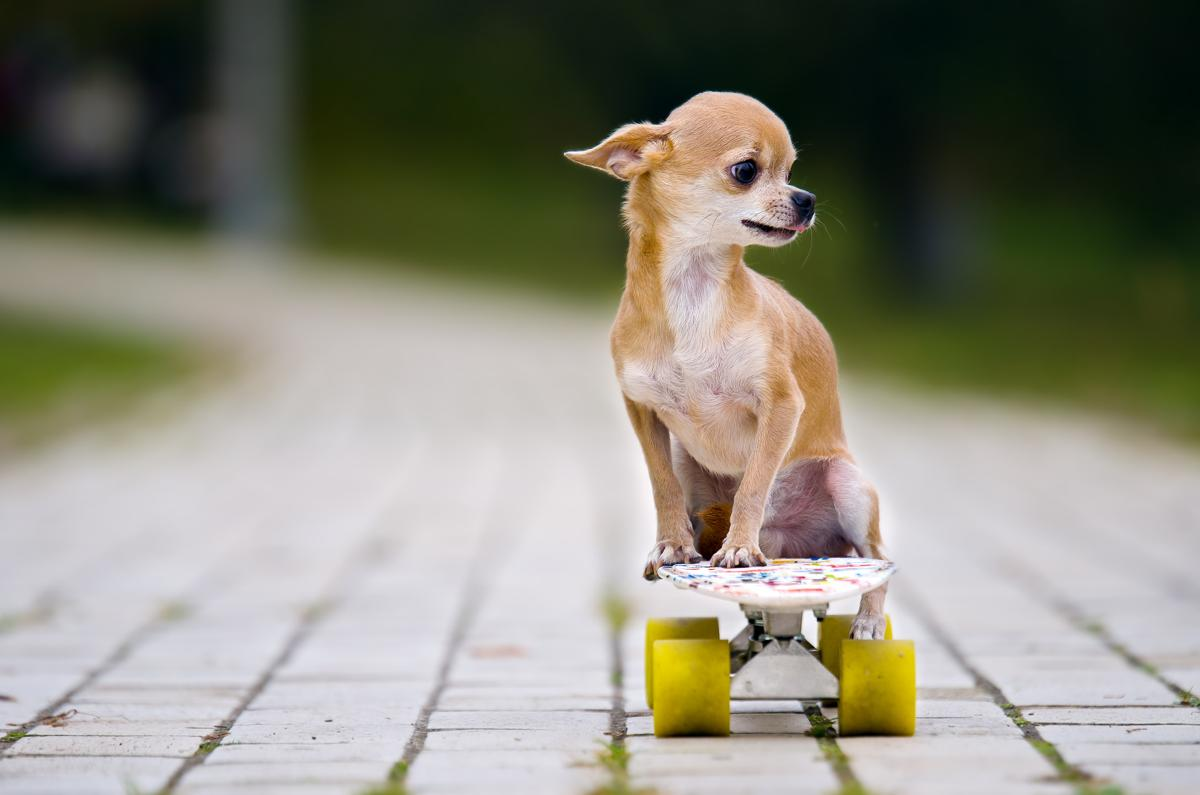
\includegraphics[width=\linewidth]{chichi.jpg}
  \caption{A Chihuahua.}
  \label{fig:chichi}
\end{figure}
%
Figure \ref{fig:chichi} shows the best kind of dog.
%
We can make lots of analysis.
%
Something about cool insight that would be interesting to Scientific Visualizaiton researchers.
%
Comparison of results to others? 
%
Major comparison to "Particle Advection Performance Over Varied Architectures and Workloads"...
%
%%%%%%%%%%%%%CONCLUSION%%%%%%%%%%%%%%%%%%%%%%%%%%%%%%%%
%%%%%%%%%%%%%%%%%%%%%%%%%%%%%%%%%%%%%%%%%%%%%%%%%%%%%%%%
\section{Conclusions and Future Work}
We studied the affects of adaptive device selection during a vtk-m Particle Advection run. 
%
We have shown that by analyzing the current workload and selecting an appropriate device, we get better performance over the traditional single-device alternatives. 
%
Our findings suggest that adaptively selecting an appropriate device can also lead to better energy efficiency, in addition to enhanced performance. 
%
We hope to get this paper published and solve world hunger while we're at it.
%
Should we do a summary of findings?

My work described in this paper highlights the performance benefits and insights that I accomplished using specifically the Particle Advection algorithm.
%
For our future work, it would be beneficial to see how this idea could be extended to other Scientific Visualizaiton algorithms.
%
For example, can we see similar performance benefits with other similar algorithms?
%
What about algorithms which have more irregular control flows or memory access patterns?
%
There are several interesting research questions that can be explored by extending this idea to other kinds of problems.
%
More on this later.
%
%%%%%%%%%%%%ACKNOWLEDGEMENTS%%%%%%%%%%%%%%%%%%%%%%%%%%%%%%%
%%%%%%%%%%%%%%%%%%%%%%%%%%%%%%%%%%%%%%%%%%%%%%%%%%%%%%
\section{Acknowledgements}
I would like to give a special thanks to the Scientific Visualization group at Oak Ridge National Labratory for their help and computational resources.
%
My work was made possible by many researchers in the group, which I very much appreciate.
%
Other thanks?

\bibliography{references} 
\bibliographystyle{alpha}
\end{document}
